\documentclass[DIV=calc,10pt,parskip=half,twocolumn]{scrartcl}
%zu ladende Pakete
\usepackage{lmodern}
\usepackage{booktabs}
\usepackage{microtype}
\usepackage{graphicx}
\usepackage{fontawesome5}

\usepackage{fontspec}
\usepackage{xcolor}
\usepackage[ngerman]{babel}
\usepackage{tcolorbox}


\setmainfont{Lora}
\definecolor{seagreen}{RGB}{0,82,76}
\definecolor{meerblau}{RGB}{0,45,116}
\definecolor{himmelblau}{RGB}{165,255,255}
\definecolor{mint}{RGB}{143,255,197}
\definecolor{violet}{RGB}{73,14,103}
\definecolor{flieder}{RGB}{205,161,255}
\definecolor{gelb}{RGB}{216,255,63}
\definecolor{bremerhavengruen}{RGB}{104,129,60}

\newfontfamily\popp{Poppins}

\setkomafont{disposition}{\color{seagreen}\fontspec{Poppins}}

%\renewcommand{\familydefault}{\sfdefault}


\author{Andi Weisen} 


\begin{document}
\title{
\vspace{-1.5em}
\begin{tcolorbox}[colframe=meerblau,top=12pt,bottom=12pt,colback=meerblau,sharp corners,halign=center]
  \popp\fontsize{40pt}{46pt}\selectfont\color{himmelblau}Spiel{\color{gelb}ereien} {\color{flieder} mit} \LaTeX{} und {\color{mint}Farben}.
\end{tcolorbox}  
\vspace{-2.5em}
}
\author{}
\date{}


\maketitle

\begin{abstract}\itshape %\bfseries
  \color{seagreen}
  Bekanntlich schrieb \glqq Weizenbaum\grqq{} das Programm Eliza~\cite{Weizenbaum1966}. 
Über Grace Hopper gibt es eine recht interessante Biographie~\cite{Beyer2009}.  
Von Knuth ist natürlich das \TeX{}-Buch zu zitieren~\cite{Knuth1984}. 
Und alle lieb(t)en \emph{Alice in Wonderland}~\cite{CarrollLewis1904}. 
\end{abstract} 

\tableofcontents 

\section{Das Ganze}
%Das ist ein neuer Absatz.

%\faGithub This is a GitHub logo.

%\faFrown[regular]

\subsection{Hinunter in den Kaninchenbau}

Alice {\bfseries fing an sich zu} langweilen; sie saß schon lange bei ihrer Schwester am
Ufer und hatte nichts zu thun. Das Buch, das ihre Schwester las, gefiel ihr
nicht; denn es waren weder Bilder noch Gespräche darin. \grqq{} Und was nützen
Bücher,\grqq{}  dachte Alice, \grqq{}ohne Bilder und Gespräche?\grqq 

Sie überlegte sich eben, (so gut es ging, denn sie war schläfrig und dumm von
der Hitze,) ob es der Mühe werth sei aufzustehen und Gänseblümchen zu pflücken,
um eine Kette damit zu machen, als plötzlich ein weißes Kaninchen mit rothen
Augen dicht an ihr vorbeirannte.

\subsection{mehr vom Ganzen}

Dies war grade nicht sehr merkwürdig; Alice fand es auch nicht sehr
außerordentlich, daß sie das Kaninchen sagen hörte: \grqq{} O weh, o weh! Ich werde zu
spät kommen!\grqq{}  (Als sie es später wieder überlegte, fiel ihr ein, daß sie sich
darüber hätte wundern sollen; doch zur Zeit kam es ihr Alles ganz natürlich
vor.) Aber als das Kaninchen seine Uhr aus der Westentasche zog, nach der Zeit
sah und eilig fortlief, sprang Alice auf; denn es war ihr doch noch nie
vorgekommen, ein Kaninchen mit einer Westentasche und einer Uhr darin zu sehen.
Vor Neugierde brennend, rannte sie ihm nach über den Grasplatz, und kam noch
zur rechten Zeit, um es in ein großes Loch unter der Hecke schlüpfen zu sehen.




\section{Tabellen und Grafiken}

Den nächsten Augenblick war sie ihm nach in das Loch hineingesprungen, ohne zu
bedenken, wie in aller Welt sie wieder herauskommen könnte.

\begin{center}
\begin{tabular}{lll}
  \toprule
   Spalte 1 &  Spalte 2 & Spalte 3\\
   \midrule
   Linksbündig & Zentriert & Rechtsbündig\\
   linksbündig & zentriert & rechtsbündig\\
   \bottomrule
\end{tabular}
\end{center}

Der Eingang zum Kaninchenbau lief erst geradeaus, wie ein Tunnel, und ging dann
plötzlich abwärts; ehe Alice noch den Gedanken fassen konnte sich schnell
festzuhalten, fühlte sie schon, daß sie fiel, wie es schien, in einen tiefen,
tiefen Brunnen.



%\begin{figure}[h!]
%  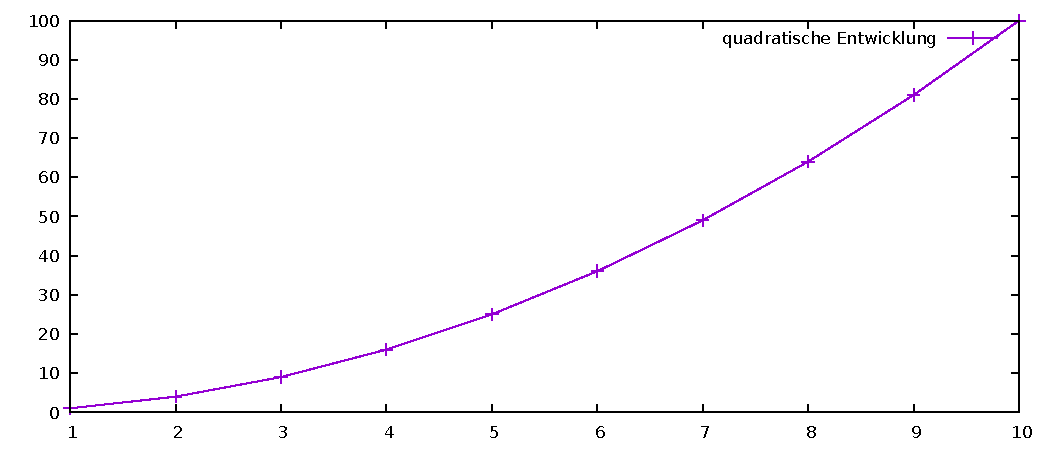
\includegraphics[width=\linewidth]{quadrat}
%  \caption{Eine Grafik}
%  \label{fig:grafikeins}
%\end{figure}


\bibliographystyle{alphadin}
\bibliography{first}
\end{document}


